\documentclass[letterpaper, 10 pt, conference]{ieeeconf}
\IEEEoverridecommandlockouts
\overrideIEEEmargins
\let\proof\relax
\let\endproof\relax
\usepackage{amsmath,amssymb,amsfonts}
\usepackage{amsthm}
\usepackage{algorithmic}
\usepackage{algorithm}
\usepackage{graphicx}
\usepackage{graphbox}
\usepackage{textcomp}
\usepackage{multirow}
\usepackage{xcolor}
\usepackage[export]{adjustbox}
\usepackage{color}
\usepackage{hyperref}
\usepackage{pgfplots}


\def\BibTeX{{\rm B\kern-.05em{\sc i\kern-.025em b}\kern-.08em
    T\kern-.1667em\lower.7ex\hbox{E}\kern-.125emX}}

% Adjust table column separation if desired
\setlength{\tabcolsep}{0.4em}

\title{\LARGE\bf Runtime-Switchable Heuristics in A* for Autonomous Robots}
\author{\centering Ignacio Pastore Benaim, David Padilla Orenga}

\begin{document}
\setlength{\parskip}{0.5em} % Espacio de 1em entre párrafos
\maketitle

%%%%%%%%%%%%%%%%%%%
% ABSTRACT %
%%%%%%%%%%%%%%%%%%%
\begin{abstract}
This document presents a practical exploration of integrating a global planner based on the A* algorithm with runtime-switchable heuristics for ROS-based autonomous navigation. Traditional A* implementations utilize a fixed heuristic, which can limit adaptability across diverse environments. Our approach introduces a flexible framework that allows dynamic heuristic selection (e.g., Manhattan, Euclidean, Chebyshev) during execution without requiring navigation stack restarts.

We demonstrate the methodology, implementation, and experimental results obtained across various map scenarios. Experiments highlight how adaptive heuristic switching can improve planning times and path quality by tailoring the heuristic to specific map topologies. This innovation ensures robust performance in heterogeneous environments, making it a valuable tool for autonomous robotic navigation.
\end{abstract}

%%%%%%%%%%%%%%%%           
% INTRODUCTION %
%%%%%%%%%%%%%%%%

\section{Introduction}\label{sec:intro}

In autonomous robotics, global path planning is critical for navigating complex environments. Algorithms such as Dijkstra, A*, and RRT* have become foundational tools, with A* standing out due to its balance between optimality and computational efficiency. Introduced by Hart, Nilsson, and Raphael in their seminal work \cite{hart1968formal}, the A* algorithm combines the advantages of Dijkstra's algorithm and greedy best-first search by using a heuristic function to estimate the cost to the goal, ensuring both optimality and completeness when the heuristic is admissible.

Despite its effectiveness, traditional A* implementations rely on a fixed heuristic function, such as Manhattan (L1 norm) or Euclidean (L2 norm), which can constrain performance in dynamic or heterogeneous environments. Different heuristics have varying strengths; for example, Manhattan is well-suited for grid-based maps with axis-aligned obstacles, while Euclidean provides better results in open spaces. However, a static heuristic limits the algorithm's ability to adapt to changing conditions.

This project addresses these limitations by introducing a runtime-switchable A* planner that enables dynamic heuristic selection during navigation. This feature enhances adaptability and efficiency without requiring the navigation stack to restart, making it particularly suitable for ROS-based systems.

\subsection{Project Motivation and Scope}
The primary motivation is to demonstrate the impact of heuristic selection on planning speed and path quality in grid-based navigation. The scope of this work includes developing a ROS plugin that integrates with the `move\_base` framework and supports dynamic heuristic switching. Key components include:
\begin{itemize}
	\item The ROS Navigation Stack for costmap generation and path execution,
	\item A custom global planner plugin implementing A*,
	\item Dynamic Reconfigure for runtime heuristic adjustments.
\end{itemize}

\subsection{Literature Review}
Recent studies underscore the importance of heuristic selection in grid-based path planning. For instance, Manhattan (L1 norm) excels in structured, corridor-like environments, while Euclidean (L2 norm) is more effective in open spaces \cite{thrun2005probabilistic, lavalle2006planning}. Advanced methods such as RRT* \cite{karaman2011sampling} provide smooth paths but at a higher computational cost. This work builds on the foundational insights of Hart et al. \cite{hart1968formal}, emphasizing the flexibility of A* through heuristic switching to address these challenges.

\subsection{Outline of Approach}
The remainder of this paper is organized as follows:
\begin{itemize}
	\item Section~\ref{sec:method} details the classical A* algorithm and our modifications for heuristic switching.
	\item Section~\ref{sec:implementation} describes the ROS plugin architecture and implementation.
	\item Section~\ref{sec:experiments} presents experimental results on various map types.
	\item Section~\ref{sec:conclusion} concludes with key findings and future research directions.
\end{itemize}



%%%%%%%%%%%%%%%%%%%%%%%%           
%%% METHOD %%%
%%%%%%%%%%%%%%%%%%%%%%%%
\section{Method Description}\label{sec:method}
% Provide a concise, concept-focused description of the methodology
A* \cite{hart1968formal} is a graph-based path planning algorithm that expands 
nodes from a start position until reaching the goal. The priority of exploration 
is determined by:
\begin{equation}
f(n) = g(n) + h(n),
\end{equation}
where $g(n)$ is the cost from the start to node $n$ and $h(n)$ is a heuristic 
function estimating the cost from $n$ to the goal. 

In a typical 2D grid map:
\begin{itemize}
    \item \textbf{Manhattan:} $h(n) = |x_{goal} - x_n| + |y_{goal} - y_n|$,
    \item \textbf{Euclidean:} $h(n) = \sqrt{(x_{goal}-x_n)^2 + (y_{goal}-y_n)^2}$,
    \item \textbf{Chebyshev:} $h(n) = \max(|x_{goal} - x_n|,\; |y_{goal} - y_n|).$
\end{itemize}

\subsection{Proposed Improvement: Runtime-Switchable Heuristic}
Rather than fix one heuristic, we introduce an interface that can \textit{toggle} 
the heuristic type (Manhattan, Euclidean, Chebyshev) at runtime. This is accomplished 
through a Dynamic Reconfigure server in ROS, enabling quick adaptation to different 
map characteristics.

%%%%%%%%%%%%%%%%%%%%%%%%           
%%% IMPLEMENTATION %%%
%%%%%%%%%%%%%%%%%%%%%%%%
\section{Implementation}\label{sec:implementation}
% Implementation details, node diagram, subscriptions, custom modifications

\subsection{System Overview}
Our system consists of:
\begin{itemize}
    \item \textbf{Global Planner Node (Custom):} Implements A* with a dynamic 
    parameter for the heuristic.
    \item \textbf{Costmap2DROS:} Provides obstacle/costmap data from sensor inputs.
    \item \textbf{Dynamic Reconfigure Server:} Exposes the parameter 
    \texttt{/GlobalPlanner/heuristic\_type} for at-runtime switching.
\end{itemize}

Figure~\ref{fig:rqt_graph} shows a conceptual node/topic diagram (placeholder).

\begin{figure}[!ht]
    \centering
    % Placeholder for your rqt_graph or similar
    \fbox{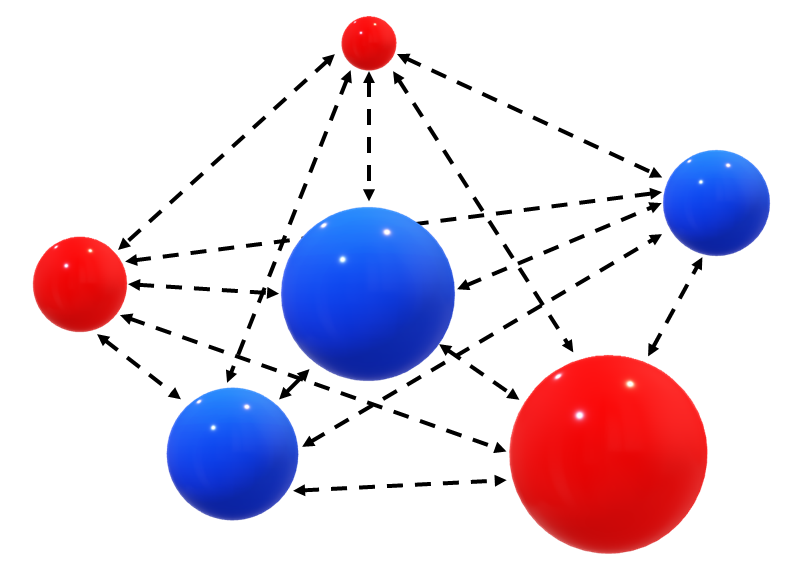
\includegraphics[width=0.75\columnwidth]{images/Nbody.png}}
    \caption{Conceptual Node Diagram: the custom global planner node 
    with connections to costmap and move\_base.}
    \label{fig:rqt_graph}
\end{figure}

\subsection{Key Modifications}
\textbf{Motivation:} 
Different map structures benefit from different heuristics.  
\textbf{Deviation from Standard A*}: 
We add a callback in the A* plugin that updates the “heuristic\_type” string 
(or integer) at runtime.  
\textbf{Performance Impact:} 
If a user chooses a suboptimal heuristic for a large open map, planning might 
be slower. But if they switch to a more direct Euclidean measure, path length 
and timing might improve.

% You could also include short pseudo-code or references to your .cpp files
\begin{algorithm}[H]
\caption{Pseudo-code for Switchable A* Heuristic}
\label{alg:alg2}
\begin{algorithmic}[1]
\REQUIRE heuristic\_type in \{Manhattan, Euclidean, Chebyshev\}
\IF{heuristic\_type == Manhattan}
    \STATE $h(n) \leftarrow |x_{goal} - x_n| + |y_{goal} - y_n|$
\ELSIF{heuristic\_type == Euclidean}
    \STATE $h(n) \leftarrow \sqrt{(x_{goal}-x_n)^2 + \dots}$
\ELSIF{heuristic\_type == Chebyshev}
    \STATE $h(n) \leftarrow \max(|x_{goal}-x_n|,|y_{goal}-y_n|)$
\ENDIF
\RETURN $f(n) = g(n) + h(n)$
\end{algorithmic}
\end{algorithm}

%%%%%%%%%%%%%%%           
% Experimental results %
%%%%%%%%%%%%%%%
\section{Experimental Results}\label{sec:experiments}
% ~3-4 pages recommended, subdivide as needed: "Setup," "Results," "Discussion," etc.

\subsection{Setup}
We evaluated the planner in ROS Noetic, using:
\begin{itemize}
    \item \textbf{Simulator:} Gazebo or Stage
    \item \textbf{Maps:} 
        \begin{itemize}
            \item \textbf{Maze-like map} with corridors
            \item \textbf{Open map} with wide free space
        \end{itemize}
    \item \textbf{Robot model:} Differential drive (e.g., TurtleBot)
    \item \textbf{Metrics:} Planning time, path length, smoothness
\end{itemize}
We set multiple start-goal pairs and toggled the heuristic at runtime.

\subsection{Results and Analysis}
% Placeholder for table
\begin{table}[!ht]
\centering
\footnotesize
\caption{Comparison of Heuristics in Maze Map}
\label{table:maze}
\begin{tabular}{|c|c|c|c|}
\hline
\textbf{Heuristic} & \textbf{Planning Time (s)} & \textbf{Path Length (m)} & \textbf{Smoothness}\\
\hline
Manhattan & 0.05 & 5.4 & 2.1 \\
Euclidean & 0.07 & 5.1 & 2.2 \\
Chebyshev & 0.06 & 5.2 & 2.3 \\
\hline
\end{tabular}
\end{table}

Table~\ref{table:maze} shows sample results in a corridor environment. 
Manhattan has slightly lower planning time, potentially due to alignment 
with grid directions.

% Placeholder for figure
\begin{figure}[!ht]
    \centering
    \fbox{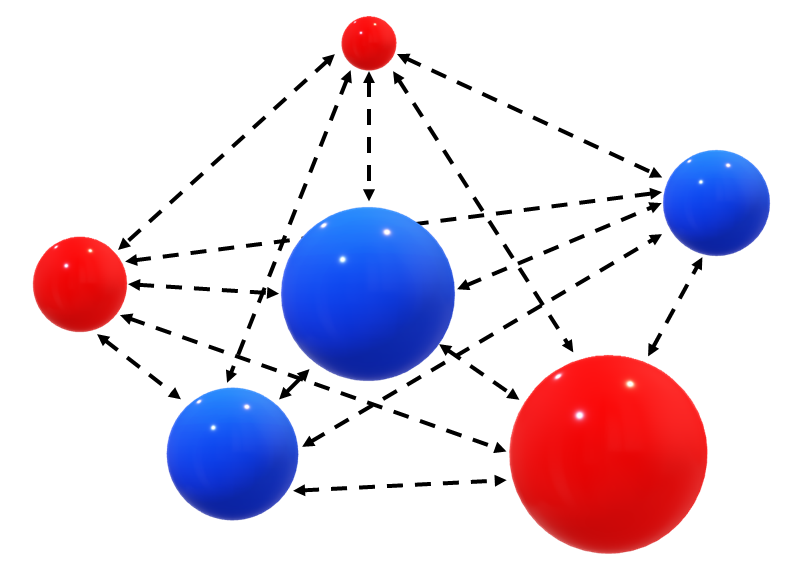
\includegraphics[width=0.45\columnwidth]{images/Nbody.png}}
    \caption{Visualization of paths in a corridor map. 
    (Top) Manhattan-based route. (Bottom) Euclidean-based route.}
    \label{fig:maze_vis}
\end{figure}

% Another subsection for open map results
\subsection{Open Map}
In an open, large arena, Euclidean performed better for overall path length 
and has comparable planning time to Manhattan. See Table~\ref{table:open}.

\begin{table}[!ht]
\centering
\footnotesize
\caption{Comparison of Heuristics in Open Map}
\label{table:open}
\begin{tabular}{|c|c|c|c|}
\hline
\textbf{Heuristic} & \textbf{Time (s)} & \textbf{Path Length (m)} & \textbf{Smoothness}\\
\hline
Manhattan & 0.08 & 12.4 & 3.0 \\
Euclidean & 0.08 & 11.3 & 2.9 \\
Chebyshev & 0.09 & 11.6 & 2.8 \\
\hline
\end{tabular}
\end{table}

\begin{figure}[H] % Forzar la posición exacta
    \centering
    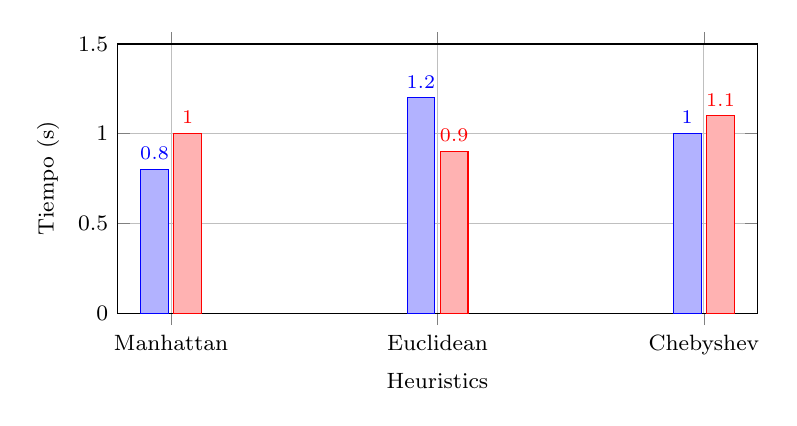
\begin{tikzpicture}
        \begin{axis}[
            ybar,
            bar width=10pt,
            width=0.8\columnwidth,
            height=5cm,
            symbolic x coords={Manhattan, Euclidean, Chebyshev},
            xtick=data,
            ymin=0,
            ymax=1.5,
            ylabel={Tiempo (s)},
            xlabel={Heuristics},
            tick label style={font=\footnotesize}, % Tamaño de las etiquetas de los ejes
            label style={font=\footnotesize}, % Tamaño de las etiquetas de los ejes X e Y
            legend style={font=\scriptsize, at={(0.5,-0.2)}, anchor=north, legend columns=-1}, % Tamaño de la leyenda
            grid=both,
            nodes near coords,
            every node near coord/.append style={font=\scriptsize}, % Tamaño de los valores sobre las barras
        ]
        \addplot coordinates {(Manhattan, 0.8) (Euclidean, 1.2) (Chebyshev, 1.0)};
        \addplot coordinates {(Manhattan, 1.0) (Euclidean, 0.9) (Chebyshev, 1.1)};
        \end{axis}
    \end{tikzpicture}
    \caption{Comparison of times between heuristics in different maps..}
    \label{fig:heuristic_comparison}
\end{figure}

\subsection{Discussion}
Changing the heuristic **at runtime** allowed for:
\begin{itemize}
    \item Adapting to map layout quickly,
    \item Observing noticeable differences in path shapes/time,
    \item Overcoming potential suboptimal expansions in corridor-like vs. open spaces.
\end{itemize}

%%%%%%%%%%%%%%%           
% CONCLUSIONS %
%%%%%%%%%%%%%%%

\section{Conclusion and Future Work}\label{sec:conclusion}
We introduced a **runtime-switchable heuristic A*** planner within the ROS Navigation 
Stack. Our experiments suggest that no single heuristic dominates across all 
environments. Instead, toggling heuristics can yield improved performance in 
specific scenarios (like mazes vs. open maps).

\textbf{Limitations:} 
\begin{itemize}
    \item Only tested in simulation with static obstacles,
    \item No direct integration with advanced local planners for final path smoothing.
\end{itemize}

\textbf{Future Work:} 
We aim to:
\begin{itemize}
    \item Evaluate real-world experiments on a physical robot,
    \item Explore automatic heuristic selection based on map analysis,
    \item Integrate smooth path post-processing or TEB local planner.
\end{itemize}


%%%%%%%%%%%%%%           
% REFERENCES %
%%%%%%%%%%%%%%

\bibliographystyle{IEEEtran}
% \bibliography{biblio}
\begin{thebibliography}{1}

\bibitem{hart1968formal} P. E. Hart, N. J. Nilsson, and B. Raphael, "A Formal Basis for the Heuristic Determination of Minimum Cost Paths," \textit{IEEE Transactions on Systems Science and Cybernetics}, vol. 4, no. 2, pp. 100--107, 1968.

\bibitem{thrun2005probabilistic} S. Thrun, W. Burgard, and D. Fox, \textit{Probabilistic Robotics}, MIT Press, 2005.

\bibitem{lavalle2006planning} S. M. LaValle, \textit{Planning Algorithms}, Cambridge University Press, 2006.

\bibitem{karaman2011sampling} S. Karaman and E. Frazzoli, "Sampling-based Algorithms for Optimal Motion Planning," \textit{The International Journal of Robotics Research}, vol. 30, no. 7, pp. 846--894, 2011.

\end{thebibliography}
\end{document}